\documentclass[11pt,a4paper]{article}

\usepackage[left=2cm,text={17cm, 24cm},top=3cm]{geometry}
\usepackage[slovak]{babel}
\usepackage[utf8]{inputenc}
\usepackage{url}
\usepackage{graphicx}
\usepackage{float}
\usepackage{pdflscape}


\bibliographystyle{czplain}

\title{manual}

\begin{document}

\begin{titlepage}
    \begin{center}
        \Huge
        \textsc{\Huge Vysoké učení technické v~Brně \\ {\huge Fakulta informačních technologií \\}}
        \vspace{\stretch{0.382}}
        {\LARGE Modelování a simulace --\ Projekt} \\ {\Huge 4. Doprava zboží nebo osob}
        \vspace{\stretch{0.618}}
    \end{center}
    {\Large \today \hfill
        xkolcu00, xdemca01}
\end{titlepage}

\tableofcontents

%----------------------NEWPAGE-------------------
\newpage
\section{Úvod}
\label{sec:UVOD}

V tejto práci sme sa rozhodli zamerať na problematiku prepravy vlakovou dopravou medzi Slovenskom a Českom na úseku Košice-Bratislava-Brno.
Tato práca vznikla na podnet slovenských študentov, študujúcich v Brne.
Vstupné dáta boli získané a agregované zo stránok cp.sk\cite{odkaz:cpsk}.
Obsahuje implementáciu modelu (\cite{odkaz:simulacia}, str. 7) železničnej dopravy na úseku Košice-Bratislava a Budapešť-Praha a jeho použitie pri určovaní pravdepodobnosti a efektivity prestupu v Bratislave na hlavnej stanici.
Dĺžka simulácie modelovaného systému (\cite{odkaz:simulacia}, str. 18) je 1 deň.

\subsection{Autori}
Autormi práce sú Robert Kolcún(xkolcu00) a Ján Demčák(xdemca01).

\subsection{Validita projektu}
\label{sec:VALIDITA}

Validita modelu (\cite{odkaz:simulacia}, str. 37) bola overená porovnávaním správania (\cite{odkaz:simulacia}, str. 24) modelu a modelovaného systému (\cite{odkaz:simulacia}, str. 18).
Štart vlakov z východzích staníc bol modelovaný podľa reálnych časov odchodov, preto boli validované s oficiálnymi údajmi zo stránok Železníc Slovenskej Republiky \cite{odkaz:slovakrail}.
Taktiež očákávané časy príchodu do jednotlivých staníc, očakávaných príchodov na dané úseky trate ako aj odchody z jednotlivých staníc boli validované podľa údajov zo stránky slovakrail.sk\cite{odkaz:slovakrail}.

Následne boli validované 1.dávkou nezávislých dát, ktoré neboli použité pri vytváraní modelovaného systému.
Za smerodajné údaje pri validácii sme považovali smerodajné odchýlky, stredné hodnoty a medián príchodov vlakov do jendotlivých úsekov.
Tak nastala fáza jemných úprav a následné 2. kolo validácie pomocou opať nových, nepoužitých dát.
Výsledné priemerné hodnoty a smerodajné odchýlky pri validácii s primeranými odchýlkami zodpovedali modelovanému systému.

\section{Rozbor tématu a použitých metod/technologií}
\label{sec:ROZBOR}

Na slovensku v súčasnosti funguje bezplatná doprava pre študentov a dôchodcov, z tohto dôvodu je pre študentov výhodnejšie využívať vlakovú dopravu narozdiel od iných spôsobov dopravy.
Veľkou nevýhodou vlakového spojenia medzi Brnom a Košicami je neexistuje priame spojenie bez nutnosti prestupu.
Jediným môžným spôsobom využitia vlakovej dopravy je teda nami modelovaný systém liniek Bratislava-Košice a Budapešť-Praha s prestupom v Bratislave v rámci vyžitia cestovania zadarmo.

Z dôvodu nastavenia dopravných liniek je ale problém vykonať tento prestup v rozumnom čase, to znamená bez niekoľko-hodinového čakania v Bratislave, kvôli krátkemu časovému intervalu na prestup, ktorý momentálne činí 5 minút (obr. \ref{pic:IMSPRESTUP}).
Pre zefektívnenie cestovania je preto významné vedieť v určitých úsekoch trate, aká je pravdepodobnosť stihnutia prestupu v Bratislave.
Obzvlášť v úseku za železničnou stanicou Žilina, kde sa nachádzajú momentálne novšie koľaje, ktoré umožňujú vlakom v prípade meškania ísť vyššou rýchlosťou a tak znížiť toto meškanie.
Určiť však hodnotu o koľko je pre bežného cestujúceho veľmi obtiažne.
V tom by mal byť prínosom práve náš navrhovaný model.

Následne sa daný cestujúci môže rozhodnúť pre predčasné vystúpenie a využitie autobusovej linky z Trenčína do Brna, ktorá by v situácii nestihnutia prestupu v Bratislave bola rýchlejšia, alebo vyžiť možnosť alternatívnej dopravy autom z Trenčína npr. pomocou služieb ako blablacar\cite{odkaz:blablacar}.

\begin{figure}[H]
    \begin{center}
    \scalebox{0.6}
    {
        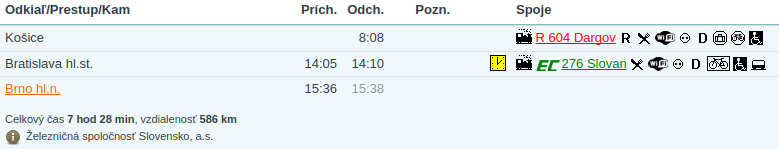
\includegraphics{imsprestup.png}
    }
    \caption{5 minútovy prestup v Bratislave}
    \label{pic:IMSPRESTUP}
    \end{center}
\end{figure}

\subsection{Popis použitých postupov pre vytvorenie modelu}
\label{sec:POSTUPI}

Simulačný model (\cite{odkaz:simulacia}, str. 44) je simulovaný pomocou diskrétnej simulácie ako systém dopravnej obsluhy (\cite{odkaz:simulacia}, str. 136).

Pre jeho implementáciu bol zvolený jazyk C++ so štandartom c++11.
Vrámci jazyka C++ bola použitá knižnica Simlib\cite{odkaz:simlib}, ktorá poskytuje nutnú funkcionalitu pre tento projekt a je pod licenciou GNU LGPL.
Súčasne je aj preferovaná a využívaná vrámci projektov na našej školy.

Pre vytvorenie samotného modelu bolo nutné určiť vhodné rozloženia a pravdepodobnosti meškania vlaku v daných úsekoch trate.
Jednotlivé meškania na daných úsekoch trate boli modelované na základe získaných dát\ref{sec:DATA} pomocou rôznych druhov rozložení.
Pre čo najvyšiu presnosť modelu, sme sa rozhodli simulovať chod vlaku v každom úseku, ku ktorému sa nám podarilo osobitne získať dáta.
To znamená že úseky medzi stanicami sú často rozdelené na menšie medziúseky.

\subsection{Popis pôvodu použitých metód/technologií}
\label{sec:POPISTECHNOLOGII}

Diskétne simulácie a knižnicu Simlib sme používali podľa popisu na prednáškach predmetu IMS.
Pri hľadaní rozložení pre meškania na daných úsekoch trate sme používali rozloženia vyučované v predmete IMS a predmete INM.
Knižnica Simlib bola stiahnutá z oficiálnych webových stránok jej autora, doktora Peringera\cite{odkaz:simlib}.
Model ani generátor vlakov nepoužíva iné prostriedky ako sú bežne dostupné v knižnici Simlib a jazyku C++.

\subsection{Zber dát}
\label{sec:DATA}

Dáta na základe ktorých bol vytvorený simulačný model boli získané zo stránok cp.sk\cite{odkaz:cpsk}, v priebehu jedného mesiaca.
Pre získanie dát sme si vytvorili script pre pravidlné sťahovanie potrebných údajov a následne ukladanie do súborov podľa dní a typu vlakov.\cite{odkaz:cpskapi}

\section{Koncepcia}
\label{sec:KONCEPCIA}

V tejto kapitole definujeme konceptuálny model, vytvorený na základe vyššie uvedených informácií a údajov určených/vypočítaných zo získaných dát.
Na základe tohto modelu bol vytvorený simulačný model.

\subsection{Zpôsob vyjádrenia konceptuálneho modelu}
\label{sec:VYJADRENIEKONCPMODELU}

Na vyjadrenie konceptuálneho modelu sme použili Petriho sieť.
Dôvodom je že abstraktný model sa skladá z prvkov ktoré typicky bývajú modelované práve Petriho sieťami.
Na úsekoch ktoré by v prípade potreby mohol vlak prekonať rýchlejšie ako má podľa jazdného poriadku, sa kontroluje či daný vlak má meškanie a následne modeluje možnosť rýchlejšej jazdy na danom úseku.
Kedže Petriho sieť zobrazujúca konceptuálny model je značne rozsiahla, a obsahuje množstvo podobných častí, rozdelili sme ju na niekoľko častí popisujúcich význačné časti konceptuálneho modelu.

\subsection{Popis konceptuálneho modelu}
\label{sec:POPISKONCMODELU}

Ako je zobrazené na obr. \ref{pic:PETSIET1}, konceptuálny model zobrazuje jeden deň, počas ktorého od času 4:08 v pravidelnom intervale 2 hodiny štartujú vlaky zo stanice v Košiciach.
Celkom ich vyštartuje 6.
Od času 7:25 štartujú vlaky zo stanice v Budapešti tiež v pravidelných intervaloch 2 hodiny.
Celkom vyrazí taktiež 6 vlakov.
Vlakov z Budapešti štartuje viac ako spomínaných 6, avšak zvyšné vlaky nie sú pre náš model dôležité pretože k nim neexistujú vlaky z linky Košice-Bratislava, na ktoré by navezovali

\begin{figure}[H]
    \begin{center}
    \scalebox{0.6}
    {
        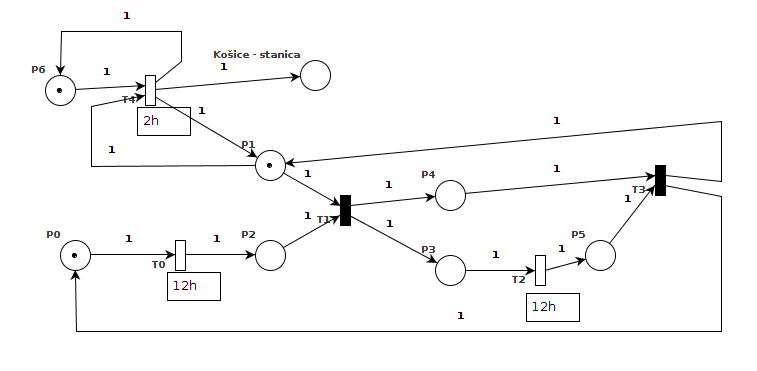
\includegraphics{Petri_net_1.png}
    }
    \caption{Generovanie vlakov počas dňa}
    \label{pic:PETSIET1}
    \end{center}
\end{figure}

Taktiež funguje nočná doprava, ktorá avšak nespadá do kategórie problému, ktorý sa snažíme riešiť kedže prestupové časy u nočných spojov sú veľmi rozdielne ako u denných liniek, a možnosti alternatívnej dopravy sú výrazne nižšie.
Priebeh daných liniek je každý deň v týždni konštantný, a zo získaných dát nebol zistený žiaden vplyv toho, v ktorý deň daný vlak ide alebo v akú dennú dobu.

Konceptuálny model predpokladá bežný deň, mimo sviatkov a dní s výrazne zvýšeným presunom ľudí, kde si situácia žiada posilové spoje, a taktiež dni obsahujúce prírodné kalamity a iné neobyčajné vplyvy prírody.
Dôvodom vynechania spomínaných stavov z daného systému je ich nízky výskyt a s tým súvisiaci malý objem dát, čo by značne ovplyvnilo presnosť a s tým aj možnú kvalitu celkového modelu.

Ako je zobrazené na  obr. \ref{pic:PETSIET2} model zohľadňuje na každom úseku trasy možnosť, že vlak získa meškanie, a taktiež možnosť závažnejšej poruchy a prípadnej kolízie s ľudskou osobou.

\begin{figure}[H]
    \begin{center}
    \scalebox{0.6}
    {
        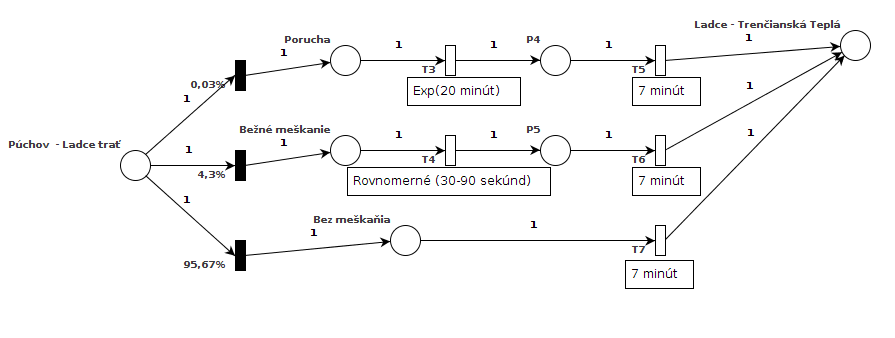
\includegraphics{Petri_net_2.png}
    }
    \caption{Príklad modelovanie meškania na úseku}
    \label{pic:PETSIET2}
    \end{center}
\end{figure}

Ako je zobrazené na  obr. \ref{pic:PETSIET3} model rozdeľuje trať na úseky medzi stanicami, kde sa dané vlaky nevedia vzájomne vyhnúť v prípapade že by jeden dobehol druhý, a stanice s určitou kapacitou kde sa vlaky v prípade poruchy môžu navzájom obehnúť.
Kapacita staníc bola volená odhadom, kedže náš model nezohľadnuje iné vlakové spojenia a nebolo tak možné určiť obsadenosť stanice v danom čase.

\begin{figure}[H]
    \begin{center}
    \scalebox{0.65}
    {
        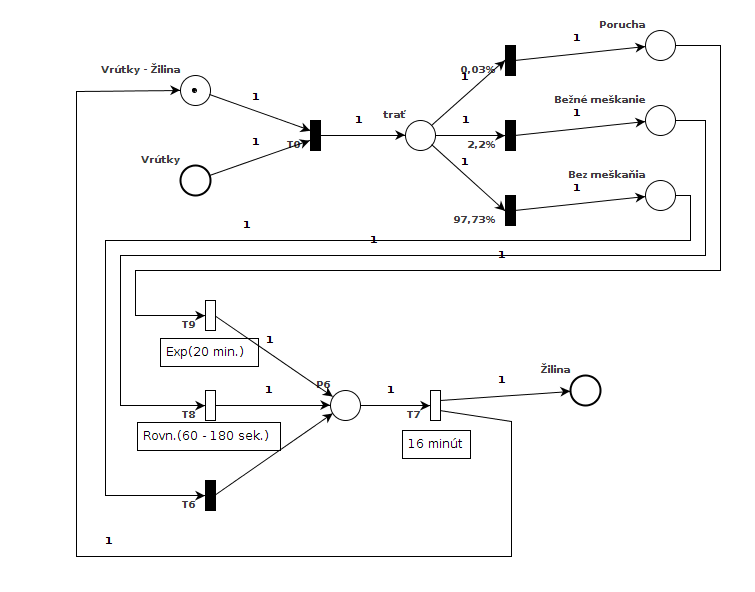
\includegraphics{Petri_net_3.png}
    }
    \caption{Príklad úseku traťe medzi 2 stanicami}
    \label{pic:PETSIET3}
    \end{center}
\end{figure}

Na linke medzi Budapešťou a Brnom, model nezohľadnuje stanice nachádzajúce sa pred stanicou Štúrovo, kvôli obmedzenosti získania dát o ceste za Slovensko-Maďarskými hranicami.
Kedže si bežný cestujúci vie zistiť informácie o meškaní vlaku až keď príde na 1.stanicu za hranicami na slovenskom územi, tak jediný údaj ktorý je pre ňho dôležitý je celkové meškanie.
Taktiež model nezohľadňuje trasu za stanicou Bratislava, keďže jeho účelom je simulovať prestup v Bratislave.

Pri príchode do stanice Bratislava daný model vyhodnocuje príchod 2 navädzujúcich vlakov na seba kde následne vyhodnotí úspešnosť prestupu.

\section{Architektura simulačního modelu/simulátoru}
\label{sec:ARCHITEKTURA}

Celá simulácia prebieha v sekundách.
Zo vstupného súboru sú načitané údaje o meškaní v jednotlivých staniciach ku každému vlaku na linke Košice-Bratislava.
Simulácia meškania na trate Budapešť-Bratislava a dá následne riešiť vzájomných rozdielom meškaní medzi týmto dvoma vlakovými linkami.
Do vstupného súboru sa taktiež zadáva počet dní, koľko krát sa má simulácia vykonať.

\subsection{Mapovanie abstraktného modelu do simulačného}
\label{sec:MAPOVANIE}

Simulácia začína vytvorením 2 objektov generátorov $(GeneratorHungary, GeneratorKe)$, kde každý generuje 1 typ vlakov, Budapešť-Praha alebo Bratislava-Košice.
Generátory následne generujú procesy $(train1, train2)$, kde každý proces odpovedá jednému vlaku.
Následne sa všetky stavy odpovedajúce úsekom trate namapujú na príslušné zariadenia $(Facility)$ a všetky stanice na sklady $(Store)$.
Kompletný zoznam tratí a staníc nájdete v tabuľke \ref{tab:USEKY}.

Na časové prechody sa používa metóda $Wait()$ na pravdepodobnostné Metóda $Random()$.

\begin{table}[H]
    \centering
    \begin{tabular}{|l|l|}
    \hline
    Ke\_KNH       & Košice-Kostoľany nad Hornádom                \\ \hline
    KNH\_Ky       & Kostoľany nad Hornádom-Kysak                 \\ \hline
    Ky\_VR        & Kysak-Výh. Ružín                             \\ \hline
    VR\_Marg      & Výh. Ružín-Margecany                         \\ \hline
    Marg\_Kr      & Margecany\_Krompachy                         \\ \hline
    Kr\_SV        & Krompachy-Spišské Vlachy                     \\ \hline
    SV\_Mar       & Spišské Vlachy-Markušovce                    \\ \hline
    Mar\_SNV      & Markušovce-Spišská Nová Ves                  \\ \hline
    SNV\_Vy       & Spišská Nová Ves-Vydrník                     \\ \hline
    Vy\_Pp        & Vydrník-Poprad-Tatry                         \\ \hline
    Pp\_Svit      & Poprad-Tatry-Svit                            \\ \hline
    Svit\_Strba   & Svit-Štrba                                   \\ \hline
    Strba\_Vych   & Štrba-Východná                               \\ \hline
    Vych\_KL      & Východná-Kráľova Lehota                      \\ \hline
    KL\_LH        & Kráľova Lehota-Liptovský Hrádok              \\ \hline
    LH\_LM        & Liptovský Hrádok-Liptovský Mikuláš           \\ \hline
    LM\_VP        & Liptovský Mikuláš-Výh. Paludza               \\ \hline
    VP\_LT        & Výh. Paludza-Liptovská Teplá                 \\ \hline
    LT\_Rk        & Liptovská Teplá-Ružomberok                   \\ \hline
    Rk\_Lub       & Ružomberok-Ľubochňa                          \\ \hline
    Lub\_Kra      & Ľubochňa-Kraľovany                           \\ \hline
    Kra\_Tur      & Kraľovany-Turany                             \\ \hline
    Tur\_Vr       & Turany-Vrútky                                \\ \hline
    Vr\_Zi        & Vrútky-Žilina                                \\ \hline
    Zi\_DH        & Žilina-Dolný Hričov                          \\ \hline
    DH\_By        & Dolný Hričov-Bytča                           \\ \hline
    By\_PB        & Bytča-Považská Bystrica                      \\ \hline
    PB\_Pu        & Považská Bystrica-Púchov                     \\ \hline
    Pu\_La        & Púchov-Ladce                                 \\ \hline
    La\_TT        & Ladce-Trenčianska Teplá                      \\ \hline
    TT\_Tn        & Trenčianska Teplá-Trenčín                    \\ \hline
    Tn\_VN        & Trenčín-Výh. Nivy                            \\ \hline
    VN\_TB        & Výh. Nivy-Trenčianske Bohuslavice            \\ \hline
    TB\_NMNV      & Trenčianske Bohuslavice-Nové Mesto nad Váhom \\ \hline
    NMNV\_Pie     & Nové Mesto nad Váhom-Piešťany                \\ \hline
    Pie\_VK       & Piešťany-VeľkéKostoľany                      \\ \hline
    VK\_Le        & Veľké Kostoľany-Leopoldov                    \\ \hline
    Le\_Bre       & Leopoldov-Brestovany                         \\ \hline
    Bre\_Tr       & Brestovany-Trnava                            \\ \hline
    Tr\_Ci        & Trnava-Cífer                                 \\ \hline
    Ci\_Se        & Cífer-Šenkvice                               \\ \hline
    Se\_VSJ       & Šenkvice-Výh.Svätý Jur                       \\ \hline
    VSJ\_Vi       & Výh. Svätý JurOdb.-Vinohrady                 \\ \hline
    Vi\_Ba        & Vinohrady-Bratislava hl stanica              \\ \hline
    \end{tabular}
    \caption{Zoznam úsekov}
    \label{tab:USEKY}
\end{table}

\section{Experimenty}
\label{sec:EXPERIMENTY}

Daný model vznikol pre určenie pravdepodobnosti stihnutia prestupu.
A pre možnosť simulovania konkrétneho meškania v danom mieste trate a následnej úspešnosti prestupu.

\subsection{Postup experimentovania}
\label{sec:POSTUPEXP}

Na modelovaný systém sme používali bez vstupných parametrov pre zistenie chovania systému v štandartných podmienkach bez do datočných informácií.
Ale aj s rôznymi hodnotami vstupných parametrov, predovšetkým sme sa zamerali na hodnoty meskania v stanici Žilina, ktorá je pre nás, ako bolo spomínané v kap.\ref{sec:ROZBOR}, najviac dôležitá.

\subsection{Jednotlivé experimenty}
\label{sec:JEDNEXP}

V prvom experimente sme v simulácií využívali žiadne vstupné parametre a určili sme percentuálnu pravdepodobnosť prestupu v stanici Bratislava.
Výsledna hodnota úspešnosti je 87.43\%.

Následne bolo v experimente č.2 zisťovaná pravepodobnosť meškania od stanice Žilina.
Postupne sme zvyšovali vstupnú hodnotu meškania pre stanicu Žilina, od počiatocnej hodnoty 60 s krokom 60 po 1400, následne sme zväčšili veľkosť kroku na 200 a následne 500.
Výsledne hodnoty experimentu sú zobrazené v obr. \ref{pic:GRAF1}.
Z grafu je možné pozorovať výraznu zmenu úspešnosti prestupu pri intervale hodnôt od 1200 do 1500.
V tomto úseku dochádza k situácií kedy už vlak nieje schopný znížit nadobudnuté meškanie na 0 kým dorazí do stanice Bratislava.
Na nasledujúcich 3 grafoch (č.\ref{pic:GRAF4}, č.\ref{pic:GRAF5}, č.\ref{pic:GRAF6}) znázorňujeme priemerne a maximálne znižovanie meškania na daných medzi úsekoch trate.
Graf č.\ref{pic:GRAF4} má počiatočné meškanie v stanici Žilina 300 sekúnd.
K priemernénu dobehnutiu meškania dojde medzi stanicami Považská Bystrica a Púchov.
Na ďalšom grafe č.\ref{pic:GRAF5} so vstupným meškaním 1000 sekúnd je možné pozorovať, že ak by vlak dosahoval maximálne hodnoty znižovania meškania tak dokáže doraziť do stanice Bratislava v čase možného prestupu.
V poslednom grafe č.\ref{pic:GRAF6} môžeme vydieť že za bežných okolností tj. ak vlak výchadzajúci z Budapešte nenaberie nadpriemerné meškanie, tak prestup nebude možný.
Dané priemerne a maximálne možné zmeny meškania za stanicou Žilina je možné vydieť v grafe č.\ref{pic:GRAF3}.

V treťom experimente sme určili priemernú percentuálnu zmenu trvania prechodu úsekom pred danou stanicou.
Výsledky sú zobrazené v grafe č.\ref{pic:GRAF2}.

\subsection{Záver experimentovania}
\label{sec:ZAVEREXP}

Pri zisku nových dát sme počítali reálnu prevdepodobnosť stihnutia prestupu a určili odchylku voči výsledku nášho systému, výsledna odchylka je 2.24\%.
Z tohto výsledku môžeme prehlásiť že systém má dôverihodné chovanie.

\section{Záver}
\label{sec:ZAVER}

Výsledna pravdepodobnosť stihnutia prestupu je 87.43\%.
Z experimentov vyplíva doporučenie že ak vlak nenaberie vačšie meškanie ako približne 12 minút, prestup bude s veľkou pravdepodobnosťou úspešný.
Ďalej z experimentov vyplýva že pri rozdiele meškania, nadvezujúcich vlakov z Košic a z Budapešti, väčšom ako 20 minút v stanici Žilina bude prestup takmer určite neuskutočnitelný.
Ako najrizikovejšie úseky na zisk meškania sú medzi stanicami Košice-Kyska, Poprad-Štrba a Vinohrady-Bratislava.

\begin{figure}[H]
    \begin{center}
    \scalebox{0.7}
    {
        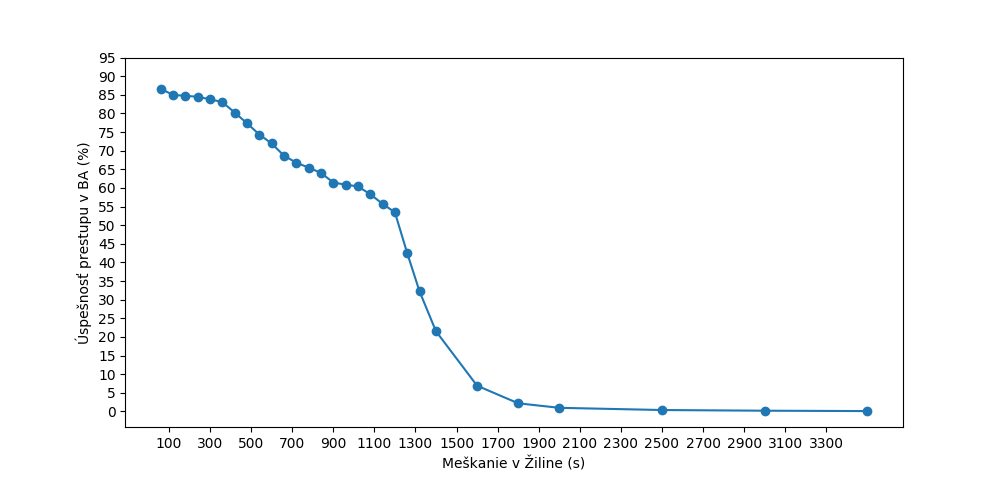
\includegraphics{Figure_1.png}
    }
    \caption{Výsledky prestupu v BA}
    \label{pic:GRAF1}
    \end{center}
\end{figure}

\begin{figure}[H]
    \begin{center}
    \scalebox{0.8}
    {
        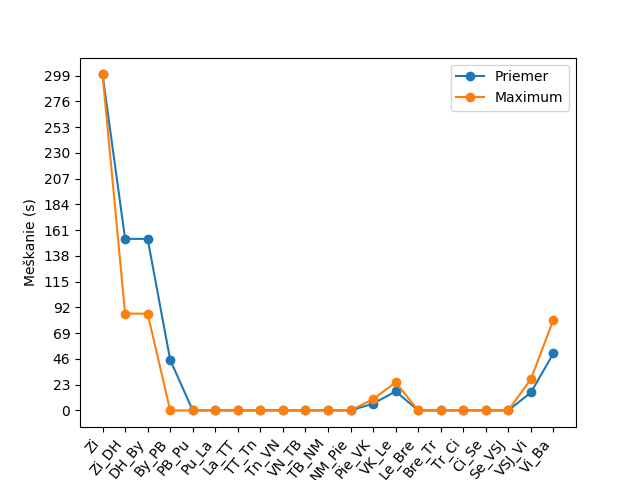
\includegraphics{Figure_4-0.png}
    }
    \caption{Znižovanie meškania od Žilini so vstupným meškaním 300 sek.}
    \label{pic:GRAF4}
    \end{center}
\end{figure}

\begin{figure}[H]
    \begin{center}
    \scalebox{0.8}
    {
        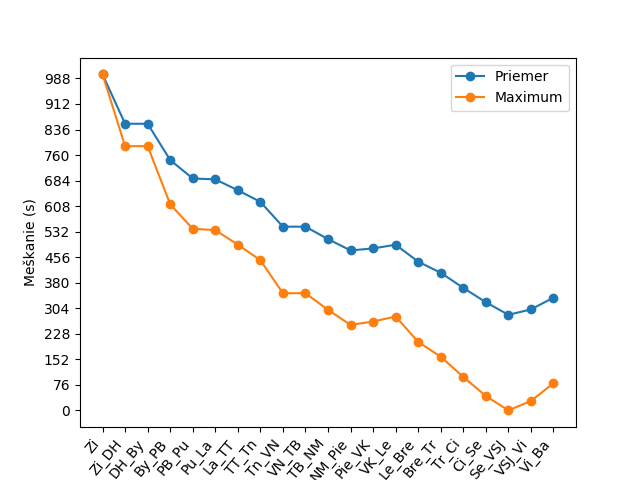
\includegraphics{Figure_4-1.png}
    }
    \caption{Znižovanie meškania od Žilini so vstupným meškaním 1000 sek.}
    \label{pic:GRAF5}
    \end{center}
\end{figure}

\begin{figure}[H]
    \begin{center}
    \scalebox{0.8}
    {
        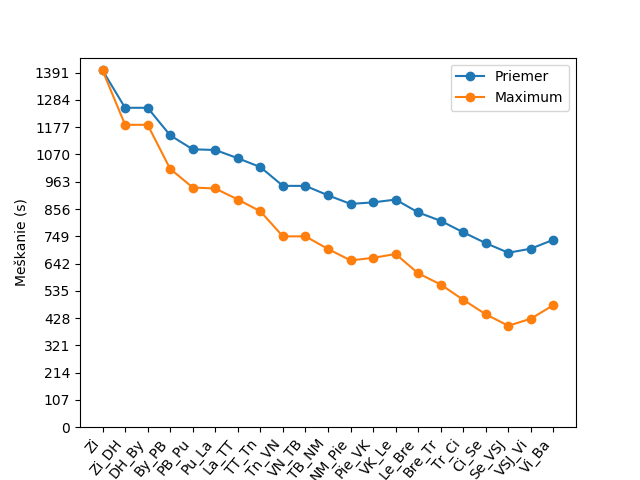
\includegraphics{Figure_4-2.png}
    }
    \caption{Znižovanie meškania od Žilini so vstupným meškaním 1400 sek.}
    \label{pic:GRAF6}
    \end{center}
\end{figure}

\begin{landscape}
    \begin{figure}[H]
        \begin{center}
        \scalebox{0.8}
        {
            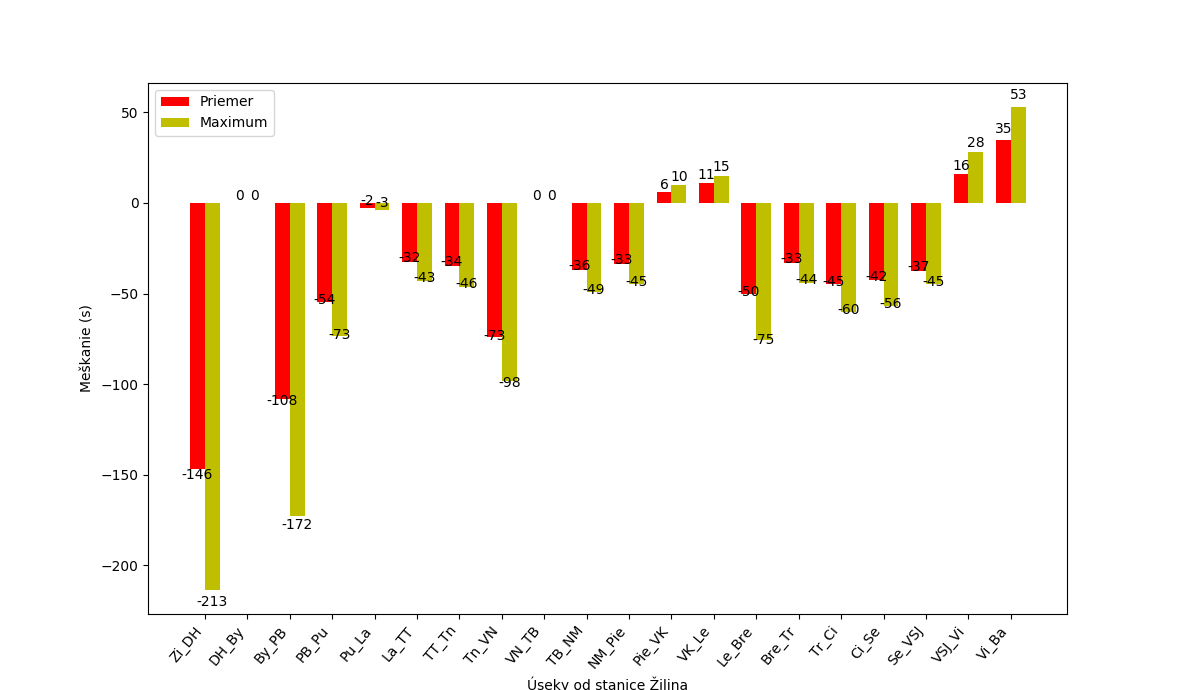
\includegraphics{Figure_3.png}
        }
        \caption{Primerna zmena meškania podľa úsekov}
        \label{pic:GRAF3}
        \end{center}
    \end{figure}
\end{landscape}

\begin{figure}[H]
    \begin{center}
    \scalebox{0.75}
    {
        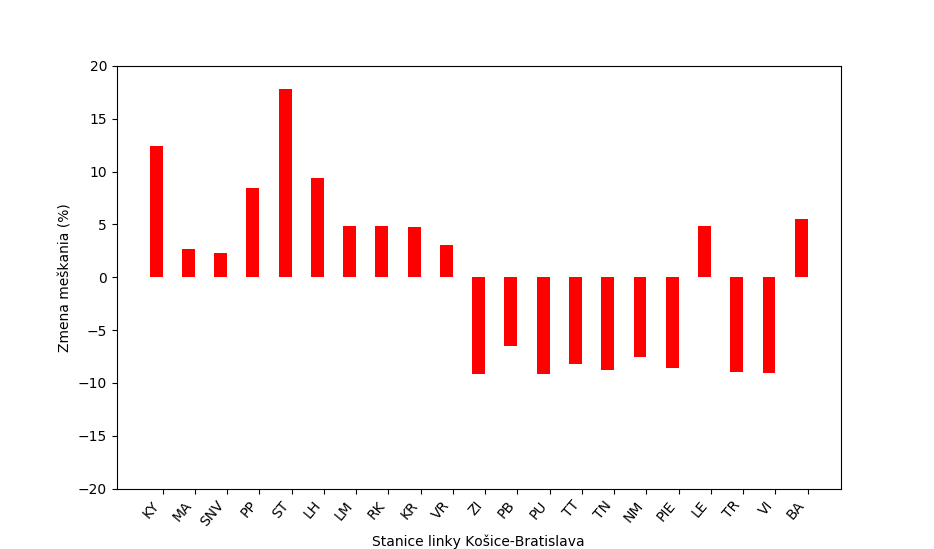
\includegraphics{Figure_2.png}
    }
    \caption{Priemerná zmena trvania prechodu úsekom pred danou stanicou}
    \label{pic:GRAF2}
    \end{center}
\end{figure}

%----------------------NEWPAGE-------------------
\newpage
\renewcommand\refname{Odkazy}
\bibliography{literatura}

\end{document}
